% Provenance (never printed): see sources/outline_sources.md (Year 3:
% energy-balance models, the one-layer model recalled; ice-albedo feedback
% and multiple equilibria; how general circulation models are built and
% evaluated).
% Brief: sources/book5/BRIEFS.md, ch. 22. Curves from
% figdata/bachelor-3/budyko_sellers.py (the zero-dimensional model and
% Budyko's latitudinal model; the brief's ebm_0d is folded into it) and
% two_layer.py. Exercise and problem values in the Book 5 scratch calculator
% calc/ch22.py. The model planet, model X and the ensemble of exercise 12 are
% invented.
\chapter{Modèles climatiques}\label{ch:b3:climate-models}

On prend le rayonnement solaire qui atteint la Terre, \qty{340}{W/m^2} en moyenne sur
le globe, et une loi pour le rayonnement infrarouge qu'elle renvoie vers l'espace, ajustée sur
trente ans d'une réanalyse des observations. On laisse l'albédo de la planète
passer de celui du sol nu et de la mer à celui de la glace à mesure que la surface se refroidit. On équilibre les deux
flux, et l'équation admet trois solutions~: une planète à
\qty{14}{\celsius}, proche de la moyenne de la Terre réelle~; une planète à
\qty{8}{\celsius}~; et une planète à \qty{-46}{\celsius}, gelée d'un pôle à
l'autre. Les modèles climatiques, depuis ces quelques lignes jusqu'aux programmes tournant sur les plus grands
calculateurs, sont des outils pour se demander quel climat une planète donnée possède, comment elle
y parvient, et comment il évolue lorsque son bilan énergétique est perturbé.
% ledger: nasa:solar-mean, data:b5-ncep-air, data:b3-ncep, budyko69:albedo

\begin{recall}
Le corps noir, la loi de Stefan--Boltzmann, l'effet de serre et le
modèle à une couche de l'atmosphère sont dans les volumes de physique~; l'albédo et
le bilan énergétique de la Terre dans les manuels du secondaire. Le rayonnement infrarouge
sortant, la température d'émission et le transport méridien de chaleur sont
dans le volume de première année, dans son chapitre sur le rayonnement et le transport de chaleur. Le
rétroaction glace--albédo et la Terre boule de neige sont dans le volume de deuxième année, dans
son chapitre sur la Terre précambrienne~; le forçage radiatif effectif, le
paramètre de rétroaction climatique $\lambda < 0$, la sensibilité climatique
à l'équilibre (ECS) et la réponse climatique transitoire (TCR) dans son chapitre
sur le changement climatique anthropique~; la prévision numérique du temps et la
prévision d'ensemble dans son chapitre sur les systèmes météorologiques. Les équations de
mouvement sur la Terre en rotation, avec l'\omterm{def:b3:gfd-foundations:hydrostatic}{approximation hydrostatique}, figurent
au chapitre~\ref{ch:b3:gfd-foundations}.
\end{recall}

\section{Le bilan énergétique d'une planète}\label{sec:b3:climate-models:zero-d}

En moyenne sur la sphère et sur une année, chaque mètre carré au sommet de
l'atmosphère reçoit $Q = S_0/4 = \qty{340}{W/m^2}$, un quart de la
éclairement solaire $S_0 = \qty{1360}{W/m^2}$. Une fraction $\alpha$, l'albédo
planétaire, est réfléchie~; le reste, $Q(1 - \alpha)$, est absorbé et
doit être renvoyé vers l'espace sous forme d'infrarouge. Un corps noir émettrait $\sigma
T^4$~; le rayonnement infrarouge sortant de la Terre (OLR) est plus faible, à cause de
l'effet de serre, et sur la gamme de températures de surface relevées sur
la Terre, elle est proche d'une droite,
\[
\text{OLR} = A + BT ,
\]
avec $T$ la température de surface en degrés Celsius. En 1969, Budyko a ajusté
une telle loi au rayonnement sortant calculé pour 260 stations, avec une correction pour
la nébulosité $n$~: $I = a + bT - (a_1 + b_1T)n$, $a = 14.0$, $b = 0.14$, $a_1 =
3.0$ et $b_1 = 0.10$ en \unit{kcal.cm^{-2}} par mois, avec une dispersion inférieure à
\qty{5}{\percent}. Pour une nébulosité moyenne de 0.5, il donne $A =
\qty{199}{W/m^2}$ et $B = \qty{1.43}{W.m^{-2}.\celsius^{-1}}$. Les \omterm{def:b3:atmospheric-dynamics:eddy}{moyennes zonales} annuelles
de la réanalyse NCEP--NCAR~1 pour 1991--2020, pondérées par la surface,
donnent $A = \qty{211.9}{W/m^2}$ et $B = \qty{1.816}{W.m^{-2}.\celsius^{-1}}$,
avec une dispersion de \qty{10}{W/m^2} autour de la droite. Ces valeurs sont utilisées
ci-dessous.
% ledger: nasa:solar-mean, budyko69:olr, data:b5-ncep-air, data:b3-ncep

\begin{definition}[Modèle de bilan d'énergie]\label{def:b3:climate-models:ebm}
Un \emph{modèle de bilan d'énergie}\index{modèle de bilan d'énergie} est un modèle
climatique qui calcule une température de surface~--- une moyenne globale unique, ou une
moyenne sur chaque latitude~--- à partir du bilan entre le rayonnement solaire absorbé, le
rayonnement infrarouge émis vers l'espace et, si la température dépend de la latitude, la
chaleur transportée vers les pôles. Dans sa forme zéro-dimensionnelle,
\[
C\,\frac{\mathrm dT}{\mathrm dt} = Q\big(1 - \alpha(T)\big) - (A + BT) ,
\]
où $C$ est la capacité thermique par unité de surface de la partie du système qui
se réchauffe avec la surface.
\end{definition}

Avec $\alpha = 0.30$, l'équilibre vaut $T = (238 - 211.9)/1.816 =
\qty{14.4}{\celsius}$~; la moyenne surfacique de la réanalyse est
\qty{14.2}{\celsius}. Un forçage $F$, comme celui d'un changement de
dioxyde de carbone, s'ajoute au membre de droite. Au voisinage d'un équilibre, la réponse est
régie par le paramètre de rétroaction climatique $\lambda$ du volume de deuxième année~:
à albédo fixé, $\lambda = -B$.
% ledger: earth:albedo, data:b5-ncep-air

\begin{theorem}[Temps de réponse d'un climat à une seule boîte]\label{thm:b3:climate-models:response}
Soit un climat à l'équilibre, et soit un forçage constant $F$ mis en route
à $t = 0$. Si l'écart $T'$ à l'équilibre obéit à $C\,\mathrm
dT'/\mathrm dt = F + \lambda T'$ avec $C > 0$ et $\lambda < 0$ constants,
alors
\[
T'(t) = -\frac{F}{\lambda}\Big(1 - \mathrm e^{-t/\tau}\Big), \qquad
\tau = -\frac{C}{\lambda} .
\]
La nouvelle position d'équilibre est $-F/\lambda$, et le climat parcourt la fraction $1
- \mathrm e^{-1} = \num{0.63}$ du chemin en un temps $\tau$.
\end{theorem}

\begin{proof}
$T'_\infty = -F/\lambda$ annule le second membre. La différence
$u = T' - T'_\infty$ obéit à $C\,\mathrm du/\mathrm dt = \lambda u$, donc $u =
u(0)\,\mathrm e^{\lambda t/C}$, avec $u(0) = F/\lambda$.
\end{proof}

La capacité thermique qui compte sur quelques années est celle de l'océan superficiel.
L'émulateur à deux couches du sixième rapport d'évaluation du
Groupe d'experts intergouvernemental sur l'évolution du climat, calé sur 44 modèles
climatiques, donne pour la couche de surface $C = \qty{8.1}{W.an.m^{-2}.\celsius^{-1}}$, la
capacité thermique d'une couche d'eau de mer de \qty{62}{m} de profondeur. Avec $\lambda = -B$, le
temps de réponse est $8.1/1.816 = \num{4.5}\text{ ans}$. Le climat réel se réchauffe aussi
l'océan profond, bien plus lentement~; la section~\ref{sec:b3:climate-models:two-layer}
l'intègre.
% ledger: ar6sm7:two-layer, teos10:cp0, data:b5-ncep-air

\section{Glace, albédo et équilibres multiples}\label{sec:b3:climate-models:multiple}

L'rétroaction glace--albédo du volume de deuxième année fait dépendre l'albédo de la
température. Prenons $\alpha = 0.62$ pour une planète dont la surface est en dessous de
$T_I = \qty{-10}{\celsius}$, l'albédo de la glace dans le modèle de Budyko, $\alpha
= 0.30$ au-dessus de $T_F = \qty{+10}{\celsius}$, et une droite entre les deux, à mesure que
la glace recule. La rampe est un choix de ce chapitre~; tout albédo qui augmente quand la
planète se refroidit donne le même tableau.
% ledger: budyko69:albedo, earth:albedo

\begin{definition}[Équilibres climatiques multiples~; bifurcation nœud-col]\label{def:b3:climate-models:multiple-equilibria}
Un modèle climatique possède \emph{équilibres climatiques multiples}\index{équilibres climatiques multiples}
lorsque, pour les mêmes conditions extérieures, il admet plus d'un
état stationnaire. Un équilibre est stable si une petite perturbation
s'en écarte en s'amortissant, instable si elle s'amplifie. Une \emph{bifurcation
nœud-col}\index{bifurcation nœud-col} est la valeur d'un paramètre pour laquelle un équilibre
stable et un équilibre instable se rejoignent et disparaissent ensemble.
\end{definition}

\begin{proposition}[Trois équilibres et leur stabilité]\label{prop:b3:climate-models:three}
Posons $N(T) = Q(1 - \alpha(T)) - (A + BT)$ pour le flux net descendant. Un
équilibre $T^*$, $N(T^*) = 0$, est stable si $N'(T^*) < 0$ et instable si
$N'(T^*) > 0$. Avec la rampe ci-dessus, $N' = -B$ sur les branches boule de neige et
sans glace, qui sont stables partout où elles existent, et $N' = -B -
Q\,\mathrm d\alpha/\mathrm dT$ sur la rampe, qui est instable lorsque $Q\,
|\mathrm d\alpha/\mathrm dT| > B$. Pour $Q = \qty{340}{W/m^2}$, le modèle possède
trois équilibres, \qty{-45.5}{\celsius} (stable), \qty{7.8}{\celsius}
(instable) et \qty{14.4}{\celsius} (stable).
\end{proposition}

\begin{proof}
Au voisinage de $T^*$, $C\,\mathrm dT'/\mathrm dt = N'(T^*)T'$, qui s'amortit si
$N'(T^*) < 0$ et s'amplifie si $N'(T^*) > 0$. Sur la rampe, $\mathrm d\alpha/
\mathrm dT = -0.32/20 = \qty{-0.016}{\celsius^{-1}}$, donc $N' = -1.816 + 340
\times 0.016 = \qty{+3.62}{W.m^{-2}.\celsius^{-1}}$. La branche boule de neige,
$T = (340\times0.38 - 211.9)/1.816 = \qty{-45.5}{\celsius}$, se situe sous
$T_I$~; la branche chaude, \qty{14.4}{\celsius}, au-dessus de $T_F$~; sur la rampe,
$340(0.54 + 0.016\,T) = 211.9 + 1.816\,T$ donne $T = \qty{7.8}{\celsius}$.
\end{proof}

\begin{omfigure}
\begin{tikzpicture}
\begin{groupplot}[group style={group size=2 by 1, horizontal sep=1.5cm},
  width=0.48\linewidth, height=0.4\linewidth,
  tick label style={font=\scriptsize}, label style={font=\small}, title style={font=\small}]
\nextgroupplot[xlabel={$T$ (\unit{\celsius})}, ylabel={flux (\unit{W/m^2})},
  xmin=-60, xmax=40, ymin=80, ymax=270, title={bilan à $Q = \qty{340}{W/m^2}$},
  legend style={font=\scriptsize, at={(0.03,0.97)}, anchor=north west}]
% computed in figdata/bachelor-3/budyko_sellers.py
\addplot[omThm, thick] table[x=T, y=asr] {figdata/out/bachelor-3-budyko_sellers-asr.dat};
\addlegendentry{lumière solaire absorbée}
\addplot[omDef, thick] table[x=T, y=olr] {figdata/out/bachelor-3-budyko_sellers-olr.dat};
\addlegendentry{$A + BT$}
\addplot[only marks, mark=*, mark size=2pt, forget plot] coordinates {(-45.55,129.2) (14.38,238.0)};
\addplot[only marks, mark=o, mark size=2pt, thick, forget plot] coordinates {(7.81,226.07)};
\node[font=\scriptsize, anchor=north west] at (axis cs:-45.55,125) {boule de neige};
\draw[black!60] (axis cs:7.81,226.07) -- (axis cs:16,200);
\node[font=\scriptsize, anchor=north west, inner sep=1pt] at (axis cs:16,200) {instable};
\nextgroupplot[xlabel={$S_0$ (\unit{W/m^2})}, ylabel={$T$ (\unit{\celsius})},
  xmin=1000, xmax=2200, ymin=-70, ymax=100, title={équilibres et hystérésis},
  scaled x ticks=false, xticklabel style={/pgf/number format/1000 sep={}}]
\addplot[black!40, densely dotted, forget plot] coordinates {(1360,-70) (1360,100)};
\addplot[omMeth, thick] table[x=S, y=T] {figdata/out/bachelor-3-budyko_sellers-eqwarm.dat};
\addplot[omThm, thick] table[x=S, y=T] {figdata/out/bachelor-3-budyko_sellers-eqcold.dat};
\addplot[black!60, thick, dashed] table[x=S, y=T] {figdata/out/bachelor-3-budyko_sellers-eqmid.dat};
\draw[->, thick, black!70] (axis cs:1314.6,8) -- (axis cs:1314.6,-45);
\draw[->, thick, black!70] (axis cs:2039.4,-8) -- (axis cs:2039.4,77);
\node[font=\scriptsize, anchor=south, black!60, fill=white, inner sep=1pt] at (axis cs:1360,84) {aujourd'hui};
\node[font=\scriptsize, omMeth, anchor=north west] at (axis cs:1700,32) {chaud};
\node[font=\scriptsize, omThm, anchor=north] at (axis cs:1620,-40) {boule de neige};
\end{groupplot}
\end{tikzpicture}

\par\smallskip{\small \omterm{def:b3:climate-models:ebm}{Modèle de bilan d'énergie} à zéro dimension avec une rampe
d'albédo de glace et la loi de rayonnement infrarouge sortant calée sur la
réanalyse NCEP--NCAR~1. À gauche, la lumière solaire absorbée et l'infrarouge émis
pour le Soleil actuel~: les deux courbes se coupent trois fois~; les points pleins
sont stables, le point creux est instable. À droite, la température d'équilibre en
fonction de la constante solaire, branches stables en trait plein, branche instable
en tirets. Affaiblir le Soleil à partir de sa valeur actuelle refroidit la planète
chaude jusqu'à ce que la branche chaude s'achève à \qty{1315}{W/m^2}, et le climat
tombe dans la boule de neige~; il y reste gelé jusqu'à ce que le Soleil atteigne
\qty{2039}{W/m^2}, où il rebondit vers une planète très chaude, bien au-delà du domaine
où la loi linéaire de rayonnement infrarouge sortant reste valable.}\label{fig:b3:climate-models:zero-d}
\end{omfigure}
% ledger: nasa:solar-mean, data:b5-ncep-air, budyko69:albedo, earth:albedo

À mesure que $Q$ diminue, l'équilibre chaud se refroidit et l'équilibre sur la rampe se
réchauffe. Ils se rejoignent au sommet de la rampe, $T = T_F$, où $Q(1 - 0.30) = A +
10B$~: $Q = \qty{328.7}{W/m^2}$, soit une constante solaire de \qty{1315}{W/m^2},
\qty{3.3}{\percent} en dessous d'aujourd'hui. C'est une \omterm{def:b3:climate-models:multiple-equilibria}{bifurcation nœud-col}~: en deçà,
le seul équilibre est la boule de neige, et le climat y tombe.
Renforcer de nouveau le Soleil ne ramène pas la planète chaude~: la branche boule de neige
ne s'achève qu'à l'endroit où sa température atteint $T_I$, $Q(1 - 0.62) = A -
10B$, pour une constante solaire de \qty{2039}{W/m^2}, \qty{50}{\percent} au-dessus
d'aujourd'hui. Entre les deux, l'état de la planète dépend de son histoire~:
le modèle présente une hystérésis. Dans le Néoprotérozoïque réel, la sortie de la
boule de neige du volume de deuxième année n'est pas venue d'un Soleil plus brillant mais
du dioxyde de carbone des volcans, qui s'accumulait pendant des millions d'années jusqu'à ce
que le forçage par effet de serre atteigne le seuil de déglaciation~; la ligne de glace
a alors reculé vers les pôles en quelques milliers d'années.
% ledger: hoffman17:hysteresis

\section{Le modèle de Budyko--Sellers}\label{sec:b3:climate-models:budyko-sellers}

Une température unique n'a pas de ligne de glace. En 1969, Budyko laisse la température
dépendre de la latitude et se demande de combien une réduction de l'ensoleillement
repousserait la glace vers l'équateur.

\begin{definition}[Modèle de Budyko--Sellers]\label{def:b3:climate-models:budyko-sellers}
Un \emph{modèle de Budyko--Sellers}\index{modèle de Budyko--Sellers} est un
\omterm{def:b3:climate-models:ebm}{modèle de bilan d'énergie} dans lequel la température annuelle moyenne $T(x)$ dépend de
$x = \sin\varphi$, où $\varphi$ est la latitude, les hémisphères étant symétriques.
En chaque latitude,
\[
C\,\frac{\partial T}{\partial t} = Qs(x)\big(1 - \alpha(x)\big) - (A + BT) - D(x) ,
\]
où $s(x)$ est l'insolation annuelle de la latitude divisée par sa moyenne
globale, $D(x)$ la divergence du transport de chaleur vers les pôles, et l'albédo
prend sa valeur de glace au-delà de la ligne de glace $x_s$, où $T$ descend sous une
température critique $T_c$. Budyko écrit $D = \beta(T - \bar T)$, un
rappel vers la moyenne globale $\bar T$~; sous forme diffusive, $D =
-\mathcal D\,\partial_x\big[(1 - x^2)\,\partial_xT\big]$.
\end{definition}

Le facteur $x = \sin\varphi$ est choisi parce que des intervalles égaux de $x$
délimitent des aires égales de la sphère, de sorte qu'une moyenne globale vaut $\int_0^1\cdot\,\mathrm
dx$. Budyko trouve $\beta = \qty{0.235}{kcal.cm^{-2}}$ par mois et par
degré, soit \qty{3.74}{W.m^{-2}.\celsius^{-1}}, à partir de la distribution observée
de la température en fonction de la latitude. Il fixe l'albédo à 0.62 sur la glace et à 0.50 à son bord,
là où la glace est brisée, et prend la ligne de glace actuelle à une latitude moyenne
de \ang{72} N~; la température critique est celle qui place le bord
à cet endroit.
% ledger: budyko69:transport, budyko69:albedo

\begin{proposition}[La ligne de glace du modèle de Budyko]\label{prop:b3:climate-models:iceline}
Soit $F(x_s) = \int_0^{x_s}s\,\mathrm dx$ la fraction de la lumière solaire qui
tombe du côté équatorial de la ligne de glace, et $\bar\alpha = \alpha_FF + \alpha_I(1 -
F)$ l'albédo moyen pondéré par la lumière solaire. Dans un état stationnaire du
modèle de Budyko,
\[
B\bar T = Q(1 - \bar\alpha) - A, \qquad
T(x) = \frac{Qs(x)\big(1 - \alpha(x)\big) - A + \beta\bar T}{B + \beta} ,
\]
et une ligne de glace en $x_s$, où $T = T_c$ avec l'albédo de bord $\alpha_e$,
exige
\[
Q(x_s) = \frac{(B + \beta)T_c + A(1 + \beta/B)}{s(x_s)(1 - \alpha_e) +
(\beta/B)\big(1 - \bar\alpha(x_s)\big)} .
\]
Une ligne de glace est stable là où $\mathrm dQ/\mathrm dx_s > 0$ et instable
là où $\mathrm dQ/\mathrm dx_s < 0$.
\end{proposition}

\begin{proof}
Intégrer le bilan stationnaire sur $0 \le x \le 1$~: le terme de transport
s'annule, car $\int_0^1(T - \bar T)\,\mathrm dx = 0$, et $\int_0^1
s(1 - \alpha)\,\mathrm dx = 1 - \bar\alpha$~; on obtient ainsi $\bar T$. Le
bilan stationnaire en chaque $x$ est alors linéaire en $T(x)$. En posant $T(x_s) = T_c$
et en remplaçant $\bar T$ par sa valeur, on obtient la dernière formule, linéaire en $Q$.
La condition de stabilité est admise~: elle découle de la linéarisation du
modèle dépendant du temps autour de l'état stationnaire.
\end{proof}

Sa signification est celle du modèle zéro-dimensionnel~: le long d'une branche
stable, un peu plus de soleil repousse la ligne de glace vers les pôles. La température à
laquelle le bord se situe aujourd'hui fixe $T_c = \qty{-12.3}{\celsius}$~; la
réanalyse donne \qty{-15.8}{\celsius} à \ang{72}, moyenne des deux
hémisphères. Le profil du modèle est plus froid que le profil observé dans les
tropiques et beaucoup plus chaud près des pôles~: un seul coefficient $\beta$ ne
peut pas ajuster l'ensemble du profil. Sa moyenne globale,
\qty{12.8}{\celsius}, et sa valeur à l'équateur, \qty{22.8}{\celsius}, sont proches de
les valeurs observées \qty{14.2}{\celsius} et \qty{25.7}{\celsius}.
% ledger: data:b5-ncep-air, data:b3-ncep, budyko69:albedo

\begin{omfigure}
\begin{tikzpicture}
\begin{groupplot}[group style={group size=2 by 1, horizontal sep=1.5cm},
  width=0.48\linewidth, height=0.42\linewidth,
  tick label style={font=\scriptsize}, label style={font=\small}, title style={font=\small}]
\nextgroupplot[xlabel={$Q/Q_0$}, ylabel={latitude de la ligne de glace (\unit{\degree})},
  xmin=0.95, xmax=1.25, ymin=-3, ymax=93, ytick={0,15,30,45,60,75,90},
  title={ligne de glace selon l'ensoleillement}, clip=false,
  scaled x ticks=false, xticklabel style={/pgf/number format/fixed, /pgf/number format/precision=2}]
% computed in figdata/bachelor-3/budyko_sellers.py
\addplot[black!40, densely dotted] coordinates {(1,-3) (1,93)};
\addplot[omMeth, thick] table[x=q, y=lat] {figdata/out/bachelor-3-budyko_sellers-icestable.dat};
\addplot[black!60, thick, dashed] table[x=q, y=lat] {figdata/out/bachelor-3-budyko_sellers-iceunstable.dat};
\addplot[omThm, thick] coordinates {(0.95,0) (1.2249,0)};
\addplot[omMeth, thick] coordinates {(1.0069,90) (1.25,90)};
\addplot[only marks, mark=*, mark size=2pt] coordinates {(1,72) (1,0) (0.9713,47.65)};
\addplot[only marks, mark=o, mark size=2pt, thick] coordinates {(1,30.15)};
\node[font=\scriptsize, anchor=west] at (axis cs:1.005,72) {aujourd'hui};
\draw[black!60] (axis cs:0.9713,47.65) -- (axis cs:1.02,50);
\node[font=\scriptsize, anchor=west, align=left] at (axis cs:1.02,50) {seuil de glaciation};
\node[font=\scriptsize, omThm, anchor=south] at (axis cs:1.06,1) {boule de neige};
\node[font=\scriptsize, omMeth, anchor=north] at (axis cs:1.15,89) {absence de glace};
\nextgroupplot[xlabel={latitude (\unit{\degree})}, ylabel={$T$ (\unit{\celsius})},
  xmin=0, xmax=90, xtick={0,15,30,45,60,75,90}, ymin=-35, ymax=32, title={température actuelle},
  legend style={font=\scriptsize, at={(0.03,0.03)}, anchor=south west}]
\addplot[omDef, thick] table[x=lat, y=tmodel] {figdata/out/bachelor-3-budyko_sellers-profile.dat};
\addlegendentry{modèle de Budyko}
\addplot[black, thick, mark=*, mark size=0.9pt] table[x=lat, y=tobs] {figdata/out/bachelor-3-budyko_sellers-obs.dat};
\addlegendentry{réanalyse}
\addplot[black!50, densely dashed] coordinates {(0,-12.26) (90,-12.26)};
\addlegendentry{$T_c$}
\end{groupplot}
\end{tikzpicture}

\par\smallskip{\small Modèle latitudinal de Budyko avec la loi du rayonnement infrarouge sortant de la
réanalyse et l'insolation de chaque latitude. À gauche, l'ensoleillement $Q/Q_0$
nécessaire pour maintenir la ligne de glace à chaque latitude~: branche stable en trait plein,
instable en tirets. Aujourd'hui, $Q/Q_0 = 1$, trois états coexistent~: la ligne de glace à \ang{72}
(stable), à \ang{30} (instable) et la boule de neige. La branche stable se termine
à son minimum, \ang{47.7} et \num{0.9713}~: avec moins de soleil à ce point, la
glace gagne jusqu'à l'équateur. À droite, la température actuelle du modèle face à la
\omterm{def:b3:atmospheric-dynamics:eddy}{moyenne zonale} annuelle de la NCEP--NCAR Reanalysis~1, 1991--2020, moyennée sur
les deux hémisphères~; la ligne de glace se situe là où la courbe du modèle, avec
l'albédo du bord, atteint $T_c$.}\label{fig:b3:climate-models:budyko}
\end{omfigure}
% ledger: data:b5-ncep-air, data:b3-ncep, budyko69:albedo, budyko69:transport

La branche stable présente un minimum. Avec ces valeurs, elle se situe à \ang{47.7},
pour $Q/Q_0 = \num{0.9713}$~: une baisse de \qty{2.87}{\percent} de l'ensoleillement
amène la glace jusqu'aux latitudes moyennes, et toute baisse supplémentaire l'envoie
l'équateur. Budyko trouve un seuil plus faible avec ses propres coefficients~: une
baisse de \qty{1.6}{\percent} amena sa glace à une latitude moyenne d'environ
\ang{50}, après quoi elle avança jusqu'à l'équateur d'elle-même et la température
moyenne chuta de plusieurs dizaines de degrés sous zéro. L'ajustement du rayonnement infrarouge
sortant et des albédos déplace le nombre~; la forme de la courbe, son minimum et l'emballement
qui le suit ne changent pas. La forme diffusive du modèle, résolue avec
des polynômes de Legendre en $x$, donne la même forme (l'exercice~\ref{exo:b3:climate-models:10}
traite une planète sans glace).
% ledger: budyko69:threshold, hoffman17:hysteresis

\section{Modèles à deux couches}\label{sec:b3:climate-models:two-layer}

Le temps de réponse du modèle à une boîte, de quelques années, est celui de
l'océan superficiel. En dessous, l'océan profond absorbe la chaleur pendant des siècles, et tant
qu'il le fait, la surface reste plus froide que son équilibre.

\begin{definition}[Modèle de bilan d'énergie à deux couches]\label{def:b3:climate-models:two-layer}
Un \emph{modèle de bilan d'énergie à deux couches}\index{modèle de bilan d'énergie à deux couches}
représente le climat par une couche de surface d'anomalie de température $T$
et de capacité thermique $C$, et par un océan profond d'anomalie de température $T_d$ et
de capacité thermique $C_d$, couplés par un coefficient d'échange de chaleur $\gamma > 0$~:
\[
C\,\frac{\mathrm dT}{\mathrm dt} = F + \lambda T - \gamma(T - T_d), \qquad
C_d\,\frac{\mathrm dT_d}{\mathrm dt} = \gamma(T - T_d) .
\]
\end{definition}

\begin{theorem}[Réponses rapide et lente]\label{thm:b3:climate-models:two-layer}
Soit $\lambda < 0$, $\gamma > 0$, $C, C_d > 0$, et soit un forçage constant
$F$ qui démarre en $t = 0$ depuis l'équilibre. Alors
\[
T(t) = -\frac{F}{\lambda}\Big(1 - a_f\,\mathrm e^{-t/\tau_f} - a_s\,\mathrm
e^{-t/\tau_s}\Big), \qquad a_f + a_s = 1 ,
\]
où $1/\tau_f$ et $1/\tau_s$ sont les racines de $r^2 - \big((\gamma -
\lambda)/C + \gamma/C_d\big)r - \lambda\gamma/(CC_d) = 0$. Lorsque $C \ll C_d$,
\[
\tau_f \approx \frac{C}{\gamma - \lambda}, \qquad
\tau_s \approx \frac{C_d(\gamma - \lambda)}{-\lambda\gamma}, \qquad
a_f \approx \frac{-\lambda}{\gamma - \lambda} .
\]
\end{theorem}

\begin{proof}
L'équilibre est $T = T_d = -F/\lambda$. Les écarts à celui-ci obéissent à
$\mathrm d\vec u/\mathrm dt = M\vec u$ avec
\[
M = \begin{pmatrix} (\lambda - \gamma)/C & \gamma/C\\ \gamma/C_d &
-\gamma/C_d\end{pmatrix}, \qquad
\operatorname{tr}M = -\frac{\gamma - \lambda}{C} - \frac{\gamma}{C_d},
\qquad \det M = \frac{-\lambda\gamma}{CC_d} > 0 ,
\]
donc les deux valeurs propres $-r$ sont réelles et négatives, $r$ vérifiant l'équation
du second degré de l'énoncé. Chaque composante de $\vec u$ est une combinaison de $\mathrm
e^{-t/\tau_f}$ et de $\mathrm e^{-t/\tau_s}$~; $T(0) = 0$ donne $a_f + a_s =
1$. Si $C \ll C_d$, la plus grande racine est proche de la trace, $(\gamma -
\lambda)/C$, et la plus petite est le déterminant divisé par celle-ci. Sur l'échelle de temps rapide,
l'océan profond n'a pas bougé, $T_d \approx 0$, et la surface
se stabilise à $F/(\gamma - \lambda)$, soit la fraction $-\lambda/(\gamma - \lambda)$
du réchauffement final~: c'est $a_f$.
\end{proof}

{\sloppy L'émulateur de l'évaluation, calibré sur 44 modèles, a $C =
\qty{8.1}{W.an.m^{-2}.\celsius^{-1}}$, $C_d = \qty{110}{W.an.m^{-2}.\celsius^{-1}}$
et $\gamma = \qty{0.62}{W.m^{-2}.\celsius^{-1}}$~; son paramètre de rétroaction est
échantillonné autour de $\lambda = \qty{-1.33}{W.m^{-2}.\celsius^{-1}}$. Ces valeurs
donnent $\tau_f = \num{4.1}\text{ ans}$ et $\tau_s = \num{262}\text{ ans}$, avec $a_f =
0.67$~: \qty{62}{\percent} du réchauffement arrive en moins d'une décennie, la majeure partie du
reste au fil des siècles. L'émulateur multiplie aussi l'échange de chaleur de la première
équation par une efficacité $\varepsilon = 1.34$, ce qui ralentit la surface
encore~; elle est fixée à 1 ici.\par}
% ledger: ar6sm7:two-layer

\begin{omfigure}
\begin{tikzpicture}
\begin{groupplot}[group style={group size=2 by 1, horizontal sep=1.4cm},
  width=0.48\linewidth, height=0.4\linewidth,
  tick label style={font=\scriptsize}, label style={font=\small}, title style={font=\small},
  ylabel={réchauffement (\unit{\celsius})}]
\nextgroupplot[xlabel={années après le saut}, xmin=0, xmax=500, ymin=0, ymax=6.6,
  title={quadruplement brutal},
  legend style={font=\scriptsize, at={(0.97,0.03)}, anchor=south east}]
% computed in figdata/bachelor-3/two_layer.py
\addplot[omDef, thick] table[x=t, y=T] {figdata/out/bachelor-3-two_layer-abrupt.dat};
\addlegendentry{surface $T$}
\addplot[omThm, thick] table[x=t, y=Td] {figdata/out/bachelor-3-two_layer-abrupt.dat};
\addlegendentry{océan profond $T_d$}
\addplot[black!60, densely dashed] coordinates {(0,5.91) (500,5.91)};
\addlegendentry{équilibre}
\nextgroupplot[xlabel={années depuis le début}, xmin=0, xmax=140, ymin=0, ymax=6.2,
  xtick={0,35,70,105,140}, title={\qty{1}{\percent} par an},
  legend style={font=\scriptsize, at={(0.03,0.97)}, anchor=north west}]
\addplot[omDef, thick] table[x=t, y=T] {figdata/out/bachelor-3-two_layer-ramp.dat};
\addlegendentry{surface $T$}
\addplot[omThm, thick] table[x=t, y=Td] {figdata/out/bachelor-3-two_layer-ramp.dat};
\addlegendentry{océan profond $T_d$}
\addplot[black!60, densely dashed] table[x=t, y expr=\thisrow{F}/1.33] {figdata/out/bachelor-3-two_layer-ramp.dat};
\addlegendentry{$-F/\lambda$}
\addplot[black!40, densely dotted, forget plot] coordinates {(70,0) (70,6.2)};
\addplot[only marks, mark=*, mark size=1.8pt, forget plot] coordinates {(70,1.987) (70,2.955)};
\node[font=\scriptsize, anchor=west] at (axis cs:72,1.75) {TCR};
\node[font=\scriptsize, anchor=east] at (axis cs:68,3.2) {ECS};
\end{groupplot}
\end{tikzpicture}

\par\smallskip{\small Le modèle à deux couches avec les paramètres moyens de
l'émulateur de la sixième évaluation et le forçage $F_{2\times} =
\qty{3.93}{W/m^2}$ d'un doublement. À gauche, un quadruplement brutal du
dioxyde de carbone~: \qty{62}{\percent} des \qty{5.9}{\celsius} finaux après 10
ans, \qty{78}{\percent} après 100 et \qty{95}{\percent} après 500.
À droite, le dioxyde de carbone augmente de \qty{1}{\percent} par an~: au doublement,
à l'année 70, la surface s'est réchauffée de \qty{1.99}{\celsius}, le TCR du
modèle, tandis que le réchauffement d'équilibre pour ce forçage, son ECS, vaut
\qty{2.95}{\celsius}~; la surface est en retard parce que l'océan profond
absorbe encore de la chaleur.}\label{fig:b3:climate-models:two-layer}
\end{omfigure}
% ledger: ar6sm7:two-layer, ipcc:erf-2xco2, ar6ch7:tcr

Le modèle donne les deux sensibilités du volume de deuxième année. Son ECS vaut
$-F_{2\times}/\lambda = 3.93/1.33 = \qty{2.95}{\celsius}$. Pendant une rampe
qui dure des décennies, l'océan profond, avec son échelle de temps de siècles, s'est à peine
réchauffé, et la surface est proche de l'équilibre rapide $T \approx F/(\gamma -
\lambda)$~: le TCR vaut environ $3.93/1.95 = \qty{2.0}{\celsius}$, contre
\qty{1.99}{\celsius} pour l'intégration. Avec l'efficacité, $\gamma$ est
remplacé par $\kappa = \varepsilon\gamma = \qty{0.84}{W.m^{-2}.\celsius^{-1}}$,
et $\text{TCR} = F_{2\times}/(\kappa - \lambda) = \qty{1.8}{\celsius}$,
la meilleure estimation retenue par le rapport, qui retient aussi une ECS de
\qty{3}{\celsius}, \emph{probable} entre 2.5 et \qty{4}{\celsius} (\emph{confiance
élevée}). L'évaluation constate que les écarts de $\gamma$ et
de $\varepsilon$ entre modèles expliquent 10 à \qty{20}{\percent} de leur
dispersion du TCR.
% ledger: ar6sm7:two-layer, ar6ch7:emulator, ar6ch7:tcr, ipcc:ecs, ipcc:erf-2xco2

Un modèle aussi simple, calé pour reproduire la température globale d'un grand
modèle, est un émulateur. L'évaluation a fait tourner un modèle climatique simple dont le module de température est
ce modèle à deux couches, sous la forme d'un ensemble d'un million de membres échantillonnés sur les
plages de ses paramètres, et a retenu les 2237 membres qui reproduisent le
réchauffement observé depuis 1850, la chaleur absorbée par l'océan, le
dioxyde de carbone de l'air et la fraction des émissions qui y reste.
% ledger: ar6sm7:two-layer, ar6ch1:esm

\section{Modèles de circulation générale}\label{sec:b3:climate-models:gcm}

Un \omterm{def:b3:climate-models:ebm}{modèle de bilan d'énergie} se voit donner ses rétroactions et son transport~; un
\omterm{def:b3:climate-models:gcm}{modèle de circulation générale} les calcule à partir des lois de la physique.

\begin{definition}[Modèle de circulation générale~; cœur dynamique~; paramétrisation]\label{def:b3:climate-models:gcm}
Un \emph{modèle de circulation générale}\index{modèle de circulation générale} (GCM)
est un modèle numérique de l'atmosphère, de l'océan, ou des deux couplés,
qui résout les équations du mouvement, de continuité et d'énergie d'un fluide sur
la Terre en rotation --- pour l'atmosphère, avec l'\omterm{def:b3:gfd-foundations:hydrostatic}{approximation
hydrostatique}, les « équations primitives » --- sur une grille tridimensionnelle
couvrant le globe, avancée pas à pas dans le temps. Son \emph{cœur
dynamique}\index{cœur dynamique} est la partie qui résout ces équations pour
les mouvements que la grille résout. Une
\emph{paramétrisation}\index{paramétrisation} représente l'effet sur
les variables résolues d'un processus plus petit qu'une maille --- nuages,
convection, turbulence, ondes de gravité --- par une formule en fonction des
variables résolues, avec des paramètres que les modélisateurs choisissent.
\end{definition}

La résolution détermine ce qu'il faut paramétrer. Les \omterm{def:b3:climate-models:gcm}{modèles de circulation générale}
de 1990 avaient des mailles d'environ \qty{500}{km} de côté~; les modèles globaux
du dernier rapport, environ \qty{100}{km}~; les modèles régionaux, de 25 à
\qty{50}{km}, et un exercice d'intercomparaison dédié a exploré des grilles globales
d'environ 50, 25 et même \qty{10}{km}. Un seul nuage convectif est beaucoup plus petit qu'une maille globale~: la convection
est paramétrée, et les modèles régionaux assez fins pour la résoudre sont désormais
inclus dans les intercomparaisons.
% ledger: ar6ch1:faq-resolution, ar6ch1:models, ar6ch1:parameterization

\begin{omfigure}
\centering
\begin{tikzpicture}[>=stealth, font=\small, x=1cm, y=1cm]
% grid of columns
\fill[omThm!8] (3.2,0) rectangle (4.8,4.2);
\foreach \i in {0,...,5} \draw[black!40] (\i*1.6,0) -- (\i*1.6,4.2);
\foreach \j in {0,...,6} \draw[black!40] (0,\j*0.7) -- (8,\j*0.7);
\fill[omMeth!25] (0,-0.25) rectangle (3.2,0);
\fill[black!25] (3.2,-0.25) rectangle (8,0);
\node[font=\scriptsize, anchor=north] at (1.6,-0.3) {océan};
\node[font=\scriptsize, anchor=north] at (5.6,-0.3) {continent};
% resolved flow
\foreach \y in {0.35,2.45,3.85} {\draw[->, omMeth, thick] (1.0,\y) -- (2.2,\y); \draw[->, omMeth, thick] (5.8,\y) -- (7.0,\y);}
% parameterised processes in the highlighted column
\draw[->, omDef, very thick] (4.0,0.55) -- (4.0,2.6);
\draw[->, omThm, thick, decorate, decoration={snake, amplitude=0.6mm, segment length=2mm, post length=1mm}] (3.45,4.6) -- (3.45,0.15);
\draw[->, omDef!70!black, thick, decorate, decoration={snake, amplitude=0.6mm, segment length=2mm, post length=1mm}] (4.55,0.15) -- (4.55,4.6);
\fill[white] (3.75,2.95) circle (0.22); \fill[white] (4.05,3.05) circle (0.27); \fill[white] (4.35,2.95) circle (0.2);
\draw[black!60, thick] (3.75,2.95) circle (0.22); \draw[black!60, thick] (4.05,3.05) circle (0.27); \draw[black!60, thick] (4.35,2.95) circle (0.2);
\draw[black!70, thick] (3.62,0.22) .. controls (3.55,0.62) and (4.1,0.62) .. (3.95,0.32) .. controls (3.85,0.15) and (3.7,0.35) .. (3.82,0.42);
% labels
\node[omMeth, font=\scriptsize, align=center, fill=white, inner sep=1pt] at (1.6,1.4) {vents résolus~:\\le cœur dynamique};
\node[font=\scriptsize, align=left, anchor=west] (c) at (8.3,3.1) {nuages};
\node[font=\scriptsize, align=left, anchor=west] (v) at (8.3,1.8) {convection};
\node[font=\scriptsize, align=left, anchor=west] (r) at (8.3,4.4) {lumière du soleil et infrarouge};
\node[font=\scriptsize, align=left, anchor=west] (t) at (8.3,0.4) {turbulence près de la surface};
\draw[black!50] (c.west) -- (4.6,3.05);
\draw[black!50] (v.west) -- (4.05,1.8);
\draw[black!50] (r.west) -- (4.6,4.4);
\draw[black!50] (t.west) -- (3.95,0.4);
\node[font=\scriptsize, black!70, anchor=west, align=left] at (8.3,-0.4) {paramétré dans la colonne};
\draw[decorate, decoration={brace, amplitude=4pt, mirror}] (3.2,-0.7) -- (4.8,-0.7)
  node[midway, below=4pt, font=\scriptsize] {une maille, environ \qty{100}{km}};
\end{tikzpicture}

\par\smallskip{\small Coupe à travers la grille d'un modèle global, non à
l'échelle. Entre les mailles, les vents et les transports de chaleur et d'humidité sont
calculés par le \omterm{def:b3:climate-models:gcm}{cœur dynamique}~; à l'intérieur de chaque colonne, les processus plus petits
que la maille --- nuages, convection, transfert du rayonnement solaire et
infrarouge, turbulence de la couche la plus basse --- sont paramétrés, à partir de
la température, de l'humidité et du vent résolus de la
colonne.}\label{fig:b3:climate-models:grid}
\end{omfigure}
% ledger: ar6ch1:faq-resolution, ar6ch1:parameterization

\begin{definition}[Modèle du système Terre]\label{def:b3:climate-models:esm}
Un \emph{modèle du système Terre}\index{modèle du système Terre} (ESM) est un \omterm{def:b3:climate-models:gcm}{modèle de
circulation générale} de l'atmosphère et de l'océan couplé à des modèles de la
banquise, de la surface continentale et de sa végétation, et du cycle du carbone, de sorte que
les concentrations des gaz à effet de serre et les propriétés de la
surface puissent répondre au climat qu'ils contribuent à fixer.
\end{definition}

Les \omterm{def:b3:climate-models:esm}{modèles du système Terre} sont les plus complexes des modèles utilisés par l'évaluation. Dans
les années 1990, les modèles couplés atmosphère--océan étaient à la pointe~;
dans les années 2010, les continents, la végétation et le cycle du carbone avaient été ajoutés, et
les modèles de calottes glaciaires sont en cours de couplage avec eux. La plupart de leurs projections sont
néanmoins réalisées avec des concentrations de gaz à effet de serre imposées~;
seuls les calculs pilotés par les émissions laissent le modèle calculer ces concentrations grâce à son cycle du carbone.
Entre les \omterm{def:b3:climate-models:ebm}{modèles de bilan d'énergie} et les \omterm{def:b3:climate-models:esm}{modèles du système Terre} se trouve une hiérarchie de modèles
de complexité intermédiaire, assez peu coûteux pour être exécutés pendant plusieurs milliers
d'années sans superordinateur.
% ledger: ar6ch1:models, ar6ch1:esm

\begin{omfigure}
\centering
\begin{tikzpicture}[>=stealth, font=\small,
  rung/.style={draw=omMeth!70, fill=omMeth!6, rounded corners=2pt, minimum height=0.85cm,
    text width=0.54\linewidth, align=left, inner sep=4pt},
  rname/.style={font=\small\bfseries, text width=0.2\linewidth, align=right, anchor=east}]
\node[rung] (e0) at (0,0) {température globale unique~; rayonnement solaire entrant, $A + BT$ sortant};
\node[rung] (e1) at (0,1.15) {température par latitude, transport vers les pôles, une ligne de glace};
\node[rung] (e2) at (0,2.3) {couche de surface et océan profond~; calé sur un grand modèle, un émulateur};
\node[rung] (e3) at (0,3.45) {atmosphère et océan sur une grille 3-D~: cœur dynamique et paramétrisations};
\node[rung] (e4) at (0,4.6) {un GCM avec banquise, continents, végétation et cycle du carbone};
\node[rname] at ([xshift=-6pt]e0.west) {EBM zéro-dimensionnel};
\node[rname] at ([xshift=-6pt]e1.west) {Budyko--Sellers};
\node[rname] at ([xshift=-6pt]e2.west) {EBM à deux couches};
\node[rname] at ([xshift=-6pt]e3.west) {GCM};
\node[rname] at ([xshift=-6pt]e4.west) {modèle du\\système Terre};
\draw[->, thick, black!60] ([xshift=10pt]e0.south east) -- ([xshift=10pt]e4.north east)
  node[midway, right, font=\scriptsize, align=left] {plus de processus,\\plus de calcul};
\end{tikzpicture}

\par\smallskip{\small L'échelle des modèles de ce chapitre. Chaque échelon
ajoute des processus qu'il avait fallu fournir au modèle inférieur~; les échelons du bas sont
assez peu coûteux pour être lancés un million de fois, les échelons supérieurs exigent
des superordinateurs.}\label{fig:b3:climate-models:ladder}
\end{omfigure}
% ledger: ar6ch1:models, ar6ch1:esm, ar6sm7:two-layer

\begin{definition}[Mise à l'équilibre]\label{def:b3:climate-models:spin-up}
La \emph{mise à l'équilibre}\index{mise à l'équilibre (d'un modèle)} d'un modèle climatique est son
intégration sous forçage constant, à partir d'un état initial, jusqu'à ce que ses
composantes lentes --- au premier rang l'océan profond et les réservoirs de carbone --- aient
cessé de dériver~; les expériences partent de l'état qu'il atteint.
\end{definition}

Le modèle à deux couches montre pourquoi une \omterm{def:b3:climate-models:spin-up}{mise à l'équilibre} est longue~: son temps caractéristique lent est
\num{262}~ans, et après trois d'entre eux, soit près de huit siècles, la
dérive représente encore \qty{5}{\percent} du déséquilibre initial. Le rapport
note que les différentes stratégies employées pour mettre les modèles à l'équilibre ont influé
sur leurs performances.
% ledger: ar6sm7:two-layer, ar6ch1:models

\begin{omfigure}
\centering
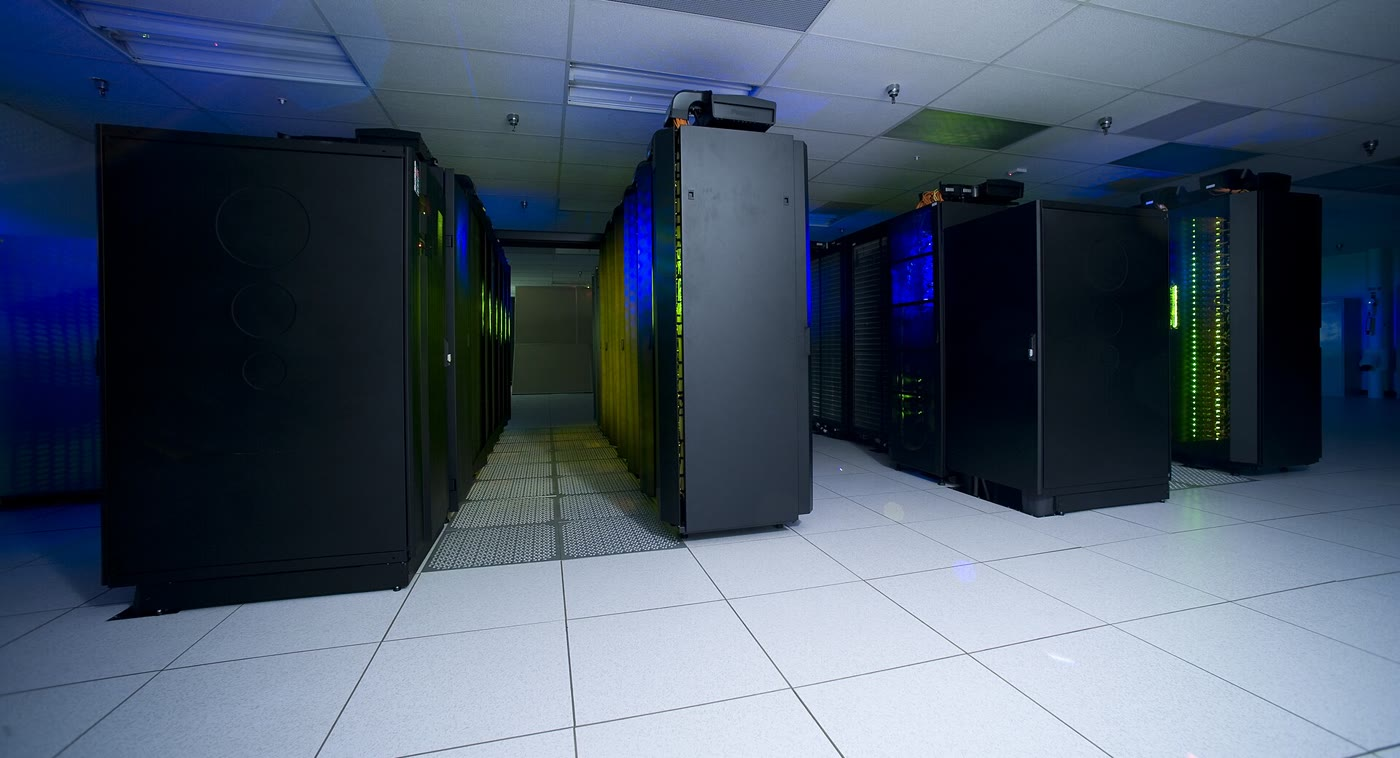
\includegraphics[width=0.7\linewidth]{images/book5/b3-nccs-supercomputer.jpg}

\par\smallskip{\small Armoires de calcul d'un superordinateur du NASA Center for
Climate Simulation, Goddard Space Flight Center, en 2010 (NASA, domaine
public). Les équations d'un modèle global sont résolues numériquement sur de tels
calculateurs à haute performance.}\label{fig:b3:climate-models:supercomputer}
\end{omfigure}
% ledger: photo:b3-nccs, ar6ch1:esm

\section{Évaluation des modèles}\label{sec:b3:climate-models:evaluation}

Un modèle est confronté au climat observé~; le problème est qu'il a
aussi été ajusté à celui-ci. Chaque \omterm{def:b3:climate-models:gcm}{paramétrisation} comporte des paramètres dont
la plage acceptable est fixée par la physique et les observations, et, à mesure que les composantes
sont assemblées, les modélisateurs les affinent jusqu'à ce que le climat simulé atteigne un
ensemble de cibles de calage~: le climat moyen --- par exemple une température moyenne
proche de la valeur observée sous l'ensoleillement actuel --- traits régionaux, ou
les tendances de la période historique. Ce n'est qu'alors que le modèle est
soumis aux intercomparaisons.
% ledger: ar6ch1:models, ar6ch1:parameterization, ar6ch1:large-ensembles

\begin{definition}[Projet d'intercomparaison de modèles]\label{def:b3:climate-models:cmip}
Un \emph{projet d'intercomparaison de modèles}\index{projet d'intercomparaison de modèles}
est un ensemble coordonné d'expériences --- mêmes forçages, mêmes
protocoles, mêmes sorties --- menés par de nombreux groupes de modélisation
avec leurs propres modèles, afin que les résultats puissent être comparés. Le
Projet d'intercomparaison de modèles couplés (CMIP) se déroule en phases successives~; sa sixième phase,
CMIP6, a fourni une source majeure de preuves pour la sixième évaluation.
\end{definition}

\begin{dated}{2021}
Parmi les 29 groupes de modélisation du CMIP6 ayant indiqué comment ils avaient calé leurs modèles, 23 n'ont pas
calé leur modèle sur le réchauffement observé pendant la période historique, et
25 n'ont pas calé leur ECS~: la sensibilité de la plupart des modèles est une
propriété émergente, non une donnée d'entrée. En moyenne, les modèles CMIP6 ont un ECS et un
TCR plus élevés que ceux de la phase précédente, et une dispersion plus large que les
fourchettes évaluées par le rapport~; dans certains modèles, cela a été attribué à la
rétroaction des nuages des latitudes moyennes et élevées. Certains des modèles les plus sensibles
reproduisent moins bien le réchauffement récent observé et les climats du passé.
Le rapport n'a donc pas tiré ses intervalles d'ECS et de TCR directement des
modèles, mais de la compréhension des processus de rétroaction,
de l'enregistrement instrumental, des climats passés et des \omterm{def:b3:climate-models:evaluation}{contraintes émergentes}~; il traite les modèles les plus sensibles comme un guide des
issues de faible probabilité et de fort impact (\emph{confiance élevée}).
\end{dated}
% ledger: ar6ch1:models, ar6ch7:cmip6-sensitivity

\begin{definition}[Grand ensemble~; contrainte émergente]\label{def:b3:climate-models:evaluation}
Un \emph{grand ensemble}\index{grand ensemble} est un ensemble de nombreuses simulations
issues d'un seul modèle, avec les mêmes forçages sur la même période, qui ne diffèrent
que par leurs états initiaux. Une \emph{contrainte
émergente}\index{contrainte émergente} est une relation, mise en évidence dans un
ensemble de modèles différents, entre une grandeur observable du
climat actuel et une grandeur du climat futur, comme l'ECS~; la
valeur observée de la première réduit alors l'intervalle de la seconde.
\end{definition}

Le climat est chaotique, si bien que de légères différences de l'état initial envoient les
membres d'un \omterm{def:b3:climate-models:evaluation}{grand ensemble} sur des trajectoires différentes~: la dispersion des
membres mesure la variabilité interne, et leur moyenne la réponse
forcée. De \omterm{def:b3:climate-models:evaluation}{grands ensembles} de plusieurs modèles ont étayé le rapport. Une
\omterm{def:b3:climate-models:evaluation}{contrainte émergente} doit reposer sur une raison physique. Sur quelques dizaines de modèles,
des milliers de grandeurs observables peuvent être testées, et certaines corréleront avec
l'ECS par hasard~; le rapport a retenu celles qui ont une base physique, beaucoup
d'entre elles concernant les nuages des tropiques, et a averti qu'un biais partagé par tous
les modèles de l'ensemble rend la méthode inopérante.
% ledger: ar6ch1:large-ensembles, ar6ch7:emergent

\begin{inthelab}[Un centre de modélisation]
\begin{minipage}[t]{0.55\linewidth}\vspace{0pt}
Dans un centre de modélisation climatique, le modèle est un programme écrit et
maintenu par une équipe~: l'atmosphère, l'océan, la banquise et les continents sont
des composantes distinctes qui échangent des flux à leurs interfaces grâce à un coupleur. Avant
chaque simulation, les forçages de l'expérience sont lus --- les concentrations de
gaz à effet de serre, les aérosols, l'occupation des sols prévue par le protocole. Le globe est
découpé en morceaux que les processeurs du superordinateur calculent côte
à côte, et un siècle de climat simulé revient sous forme d'une grande archive de
champs. Les scientifiques les affichent sur des écrans, les comparent aux
réanalyses et aux enregistrements satellitaires, et envoient les sorties standard aux
archives de l'intercomparaison, où d'autres groupes les comparent aux leurs.
\end{minipage}\hfill
\begin{minipage}[t]{0.42\linewidth}\vspace{0pt}
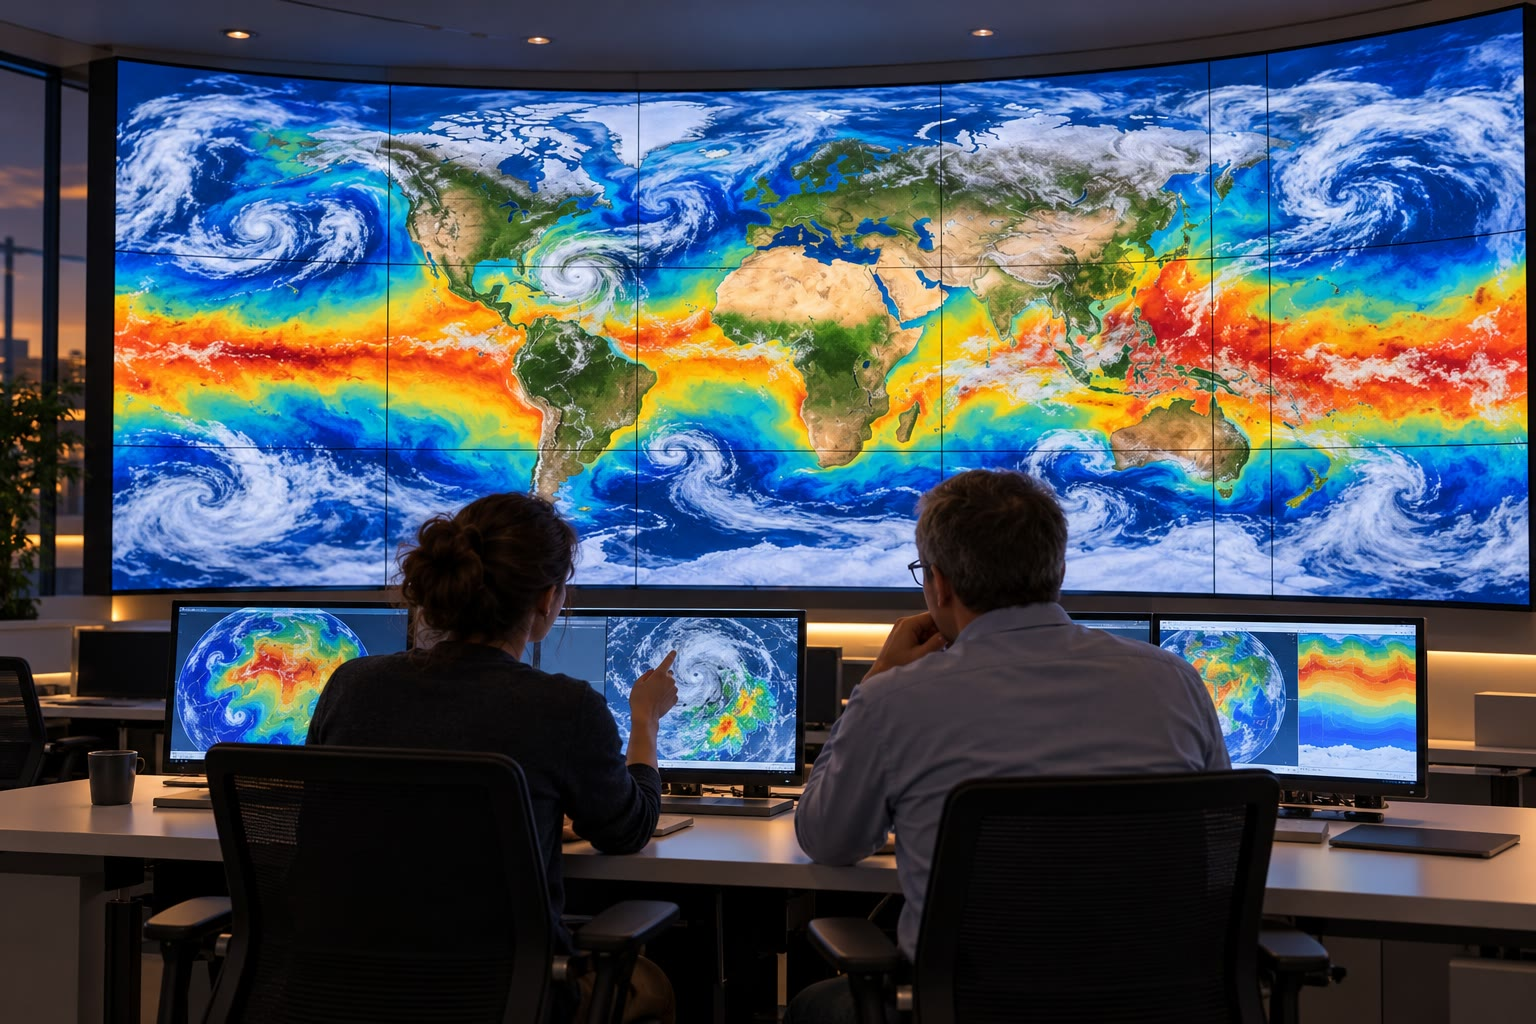
\includegraphics[width=\linewidth]{images/book5/ai/b3-model-centre.jpg}

{\scriptsize Deux scientifiques devant un mur d'écrans affichant des champs globaux
d'une simulation du modèle (Illustration générée par IA).}
\end{minipage}
\end{inthelab}
% ledger: ar6ch1:esm, ar6ch1:models

\section{Exercices}

\begin{exercise}[$\star$]\label{exo:b3:climate-models:1}
La loi de Budyko pour le rayonnement infrarouge sortant s'écrit $I = a + bT - (a_1 + b_1T)n$, avec $a = 14.0$, $b =
0.14$, $a_1 = 3.0$, $b_1 = 0.10$, en \unit{kcal.cm^{-2}} par mois et $T$
en \unit{\celsius}. Pour une nébulosité $n = 0.5$, calculer $A$ et $B$, et
les convertir en \unit{W/m^2} et \unit{W.m^{-2}.\celsius^{-1}}, un mois valant
un douzième d'année de 365.25 jours. Quel rayonnement infrarouge sortant la loi donne-t-elle à
\qty{15}{\celsius}~?
\end{exercise}
% ledger: budyko69:olr

\begin{exercise}[$\star$]\label{exo:b3:climate-models:2}
Avec $Q = \qty{340}{W/m^2}$, $A = \qty{211.9}{W/m^2}$ et $B =
\qty{1.816}{W.m^{-2}.\celsius^{-1}}$, calculer la température d'équilibre
pour un albédo de 0.30 puis de 0.31. De combien une hausse de 0.01
de l'albédo refroidit-elle cette planète~?
\end{exercise}

\begin{exercise}[$\star$]\label{exo:b3:climate-models:3}
Calculer la capacité thermique par mètre carré d'une couche de mélange d'eau de mer
de \qty{60}{m} de profondeur, $\rho = \qty{1025}{kg/m^3}$ et $c_p = \qty{3992}{J.kg^{-1}.K^{-1}}$,
en \unit{J.m^{-2}.K^{-1}} et en \unit{W.an.m^{-2}.K^{-1}}. Calculer le temps de réponse
associé au \cref{thm:b3:climate-models:response} pour $\lambda = -B =
\qty{-1.816}{W.m^{-2}.\celsius^{-1}}$ et pour $\lambda =
\qty{-1.33}{W.m^{-2}.\celsius^{-1}}$.
\end{exercise}
% ledger: teos10:cp0

\begin{exercise}[$\star$]\label{exo:b3:climate-models:4}
Pour le modèle à deux couches avec $\lambda = \qty{-1.33}{W.m^{-2}.\celsius^{-1}}$,
$\gamma = \qty{0.62}{W.m^{-2}.\celsius^{-1}}$ et $F_{2\times} =
\qty{3.93}{W/m^2}$, calculer la sensibilité climatique à l'équilibre (ECS), la réponse climatique transitoire approchée (TCR) $F_{2\times}/
(\gamma - \lambda)$, et leur rapport.
\end{exercise}
% ledger: ar6sm7:two-layer, ipcc:erf-2xco2

\begin{exercise}[$\star\star$]\label{exo:b3:climate-models:5}
Dans le modèle zéro-dimensionnel du texte, prendre une constante solaire de
\qty{1340}{W/m^2}. Trouver les trois équilibres et la pente $N'(T)$ du
flux net en chacun~; lesquels sont stables~?
\end{exercise}

\begin{exercise}[$\star\star$]\label{exo:b3:climate-models:6}
Modifier la rampe d'albédo du texte~: $\alpha = 0.62$ en dessous de \qty{-20}{\celsius},
$0.30$ au-dessus de \qty{0}{\celsius}, linéaire entre les deux. Conserver $A$ et $B$. Pour quelle constante solaire
la branche chaude se termine-t-elle, et de combien de pour cent cette valeur est-elle
inférieure à \qty{1360}{W/m^2}~? Pour quelle constante solaire la boule de neige fond-elle~?
Qu'est-ce qui fixe la taille du seuil~?
\end{exercise}

\begin{exercise}[$\star\star$]\label{exo:b3:climate-models:7}
Une planète modèle ayant les paramètres du texte se trouve à l'état de boule de neige.
(a)~Quelle est sa température avec la constante solaire actuelle~? (b)~En gardant le Soleil tel qu'il est, quel forçage $F$
ferait remonter la température de la boule de neige à
\qty{-10}{\celsius}~? Combien de fois le forçage d'un doublement du dioxyde de carbone,
\qty{3.93}{W/m^2}, représente-t-il~? (c)~Une fois la glace disparue, où la planète
se stabilise-t-elle si le forçage est ensuite supprimé~?
\end{exercise}
% ledger: ipcc:erf-2xco2, hoffman17:hysteresis

\begin{exercise}[$\star\star$]\label{exo:b3:climate-models:8}
Le modèle X, un modèle à deux couches inventé, a $C = 7.0$ et $C_d =
\qty{90}{W.an.m^{-2}.\celsius^{-1}}$, $\gamma = 0.70$ et $\lambda =
\qty{-1.10}{W.m^{-2}.\celsius^{-1}}$. Calculer ses deux échelles de temps exactement
et avec les approximations du \cref{thm:b3:climate-models:two-layer}, la
fraction $a_f$, sa sensibilité climatique à l'équilibre (ECS) et sa réponse climatique transitoire approchée (TCR).
\end{exercise}

\begin{exercise}[$\star\star$]\label{exo:b3:climate-models:9}
Dans le modèle de Budyko du texte, $\bar T = \qty{12.81}{\celsius}$, $\beta =
\qty{3.74}{W.m^{-2}.\celsius^{-1}}$, la ligne de glace à \ang{72}, $s = 1.221$
à l'équateur et $0.506$ au pôle, $\alpha = 0.30$ et $0.62$.
Calculer la température à l'équateur et au pôle, ainsi que la chaleur
$\beta(T - \bar T)$ que le transport retire ou apporte à chaque
mètre carré en ces lieux.
\end{exercise}

\begin{exercise}[$\star\star\star$]\label{exo:b3:climate-models:10}
Une planète sans glace ($\alpha = 0.30$ partout) subit le transport diffusif
$D = -\mathcal D\,\partial_x[(1 - x^2)\partial_xT]$ et l'insolation
$s(x) = 1 + s_2P_2(x)$, $P_2 = (3x^2 - 1)/2$. (a)~Montrer que
$\partial_x[(1 - x^2)\partial_xP_2] = -6P_2$. (b)~Montrer que $T = T_0 +
T_2P_2(x)$ est une solution stationnaire, avec $T_0 = (Q(1 - \alpha) - A)/B$ et
$T_2 = Qs_2(1 - \alpha)/(B + 6\mathcal D)$. (c)~L'insolation de la réanalyse donne
$s_2 = \num{-0.476}$. Sans transport, quelle serait la différence de température
entre équateur et pôle~? (d)~Quelle valeur de $\mathcal D$ donne
la différence observée, \qty{55.3}{\celsius}~?
\end{exercise}
% ledger: data:b3-ncep, data:b5-ncep-air

\begin{exercise}[$\star\star\star$]\label{exo:b3:climate-models:11}
(a)~Écrire le trinôme du \cref{thm:b3:climate-models:two-layer} sous la forme $r^2 -
\Sigma r + \Pi = 0$ et montrer que, si $4\Pi \ll \Sigma^2$, ses racines sont
voisines de $\Sigma$ et de $\Pi/\Sigma$. (b)~Pour un forçage $F = kt$ croissant
linéairement, montrer que, dès que $t \gg \tau_f$ et tant que $T_d$ reste petit,
$T \approx kt/(\gamma - \lambda)$~; en déduire la réponse climatique transitoire approchée. (c)~Vérifier
les valeurs du texte~: $\Sigma$, $\Pi$, les deux échelles de temps et le rapport
$4\Pi/\Sigma^2$.
\end{exercise}
% ledger: ar6sm7:two-layer

\begin{exercise}[$\star\star\star$]\label{exo:b3:climate-models:12}
Un ensemble fictif de huit modèles donne une observable $X$ du
climat actuel et leur sensibilité climatique à l'équilibre (ECS)~:
\begin{center}
\begin{tabular}{l*{8}{c}}
\hline
$X$ & 0.2 & 0.5 & 0.6 & 0.8 & 1.0 & 1.1 & 1.3 & 1.5\\
ECS (\unit{\celsius}) & 2.3 & 2.7 & 3.1 & 3.2 & 3.8 & 3.9 & 4.4 & 4.6\\
\hline
\end{tabular}
\end{center}
(a)~Calculer la moyenne et l'écart type de l'ECS de
l'ensemble. (b)~Ajuster ECS $= a + bX$ par moindres carrés~; calculer la corrélation
et l'écart type des résidus. (c)~L'observation $X$ vaut $0.7
\pm 0.1$. Quelle sensibilité la contrainte donne-t-elle, et avec quelle dispersion~?
(d)~Qu'est-ce qui pourrait faire douter de cette contrainte~?
\end{exercise}
% ledger: ar6ch7:emergent

\section{Problème~: à quelle distance de la Terre boule de neige~?}

\begin{problem}[{Problème du week-end --- équilibres, stabilité et
seuil de glaciation d'une planète modèle}]
\label{pb:b3:climate-models:1}
Une planète modèle a pour constante solaire actuelle $S_0 = \qty{1360}{W/m^2}$ et la
loi de rayonnement infrarouge sortant (OLR) $A + BT$ avec $A = \qty{211.9}{W/m^2}$ et $B =
\qty{1.816}{W.m^{-2}.\celsius^{-1}}$. Son albédo vaut 0.62 en dessous de
\qty{-10}{\celsius}, 0.30 au-dessus de \qty{+10}{\celsius}, linéaire entre les deux, et
sa capacité thermique surfacique $C = \qty{8.1}{W.an.m^{-2}.\celsius^{-1}}$. Prendre
$\sigma = \qty{5.670e-8}{W.m^{-2}.K^{-4}}$.

\medskip\noindent\textbf{Partie I --- La planète à l'équilibre.}
\begin{enumerate}
\item Calculer l'éclairement solaire moyen $Q_0$ par mètre carré de la planète, et
  expliquer le facteur.
\item Calculer l'éclairement absorbé pour un albédo de 0.30, et le rayonnement infrarouge sortant à
  \qty{15}{\celsius}.
\item Calculer l'équilibre chaud.
\item Calculer l'équilibre boule de neige, et vérifier qu'il se situe sur la
  branche glacée.
\item Calculer le troisième équilibre, sur la rampe d'albédo.
\item Calculer la température d'émission qui renvoie l'éclairement absorbé
  vers l'espace comme un corps noir, et la comparer à l'équilibre chaud.
\end{enumerate}

\medskip\noindent\textbf{Partie II --- Stabilité et temps.}
\begin{enumerate}[resume]
\item Calculer la pente $N'(T)$ du flux net à chaque équilibre, et dire
  lesquels sont stables.
\item Un petit écart à l'équilibre intermédiaire croît comme $\mathrm
  e^{t/\tau}$. Calculer $\tau$.
\item Calculer le temps de réponse de l'équilibre chaud.
\item Un forçage de \qty{3.93}{W/m^2}, celui d'un doublement du dioxyde de carbone,
  est imposé brusquement. Calculer le réchauffement à l'équilibre, et le comparer
  à la sensibilité climatique à l'équilibre (ECS) évaluée pour le climat réel.
\item Combien de temps le modèle met-il pour atteindre \qty{95}{\percent} du
  réchauffement~? Pourquoi le climat réel met-il plus de temps~?
\end{enumerate}

\medskip\noindent\textbf{Partie III --- La bifurcation nœud-col.}
\begin{enumerate}[resume]
\item Quand le Soleil faiblit, à quelle température l'équilibre chaud rejoint
  l'équilibre intermédiaire~? Calculer $Q$ à cette température.
\item Calculer la constante solaire à la bifurcation, et la baisse par rapport à
  aujourd'hui, en pourcentage.
\item Juste en dessous, où le climat se dirige-t-il~? Calculer sa température.
\item Calculer la constante solaire à laquelle la boule de neige fond, et la hausse
  par rapport à aujourd'hui, en pourcentage.
\item Esquisser la boucle décrite par la température lorsque $S_0$ est abaissée
  sous la bifurcation, puis ramené à \qty{1360}{W/m^2}.
\end{enumerate}

\medskip\noindent\textbf{Partie IV --- La ligne de glace.} Doter la planète
du modèle latitudinal de Budyko, avec $\beta = \qty{3.739}{W.m^{-2}.\celsius^{-1}}$,
un albédo de glace de 0.62 au-delà de la ligne de glace côté pôles, 0.30 côté équateur, 0.50 à
la limite, et l'insolation de la réanalyse~:
\begin{center}
\begin{tabular}{lccccccc}
\hline
latitude & \ang{0} & \ang{30} & \ang{40} & \ang{47.5} & \ang{55} & \ang{60} & \ang{72}\\
$s(x_s)$ & 1.2211 & 1.0730 & 0.9647 & 0.8688 & 0.7650 & 0.6947 & 0.5643\\
$F(x_s)$ & 0 & 0.5865 & 0.7324 & 0.8192 & 0.8863 & 0.9205 & 0.9738\\
\hline
\end{tabular}
\end{center}
\begin{enumerate}[resume]
\item Avec la ligne de glace à \ang{72}, calculer l'albédo moyen $\bar\alpha$
  et la température moyenne $\bar T$.
\item Calculer la température critique $T_c$ qui place la limite à
  \ang{72} aujourd'hui, et la comparer à la réanalyse, \qty{-15.8}{\celsius}.
\item Calculer le numérateur de $Q(x_s)$ dans la \cref{prop:b3:climate-models:iceline}
  et le rapport $\beta/B$.
\item Calculer $Q(x_s)/Q_0$ pour la ligne de glace à \ang{30}, \ang{40},
  \ang{47.5}, \ang{55} et \ang{60}.
\item Où se trouve le minimum de ces valeurs~? Quelles lignes de glace sont stables~?
\item Avec le Soleil actuel, quelle autre ligne de glace le modèle autorise-t-il, et est-elle
  stable~? La boule de neige est-elle possible aujourd'hui~? (Utiliser la colonne \ang{0}.)
\item Comparer le seuil du modèle latitudinal à celui de la partie~III
  et à celui de Budyko, \qty{1.6}{\percent}, et la latitude de la glace au
  seuil avec son \ang{50}.
\item Donner, à deux chiffres significatifs, la baisse de la constante solaire, en
  pourcentage, qui fait basculer la planète modèle dans la glaciation.
\end{enumerate}
\end{problem}
% ledger: nasa:solar-mean, data:b5-ncep-air, data:b3-ncep, budyko69:transport, budyko69:albedo, budyko69:threshold, ipcc:ecs, const:sigma
